\documentclass[10pt,letterpaper]{article}
\usepackage[margin=0.7in,headheight=14pt]{geometry}
\usepackage[T1]{fontenc}
\usepackage{lmodern,amsmath,amssymb,booktabs,graphicx,xcolor}
\usepackage[colorlinks=true,urlcolor=blue,linkcolor=blue]{hyperref}
\hypersetup{pdftitle={Homework 2 Solutions},pdfauthor={Ruochen Wang}}
\pagestyle{myheadings}\markright{\small Ruochen Wang\quad |\quad Foundations of Machine Learning and AI\quad |\quad HW2}
\setlength{\parindent}{0pt}\setlength{\parskip}{6pt}
\setlength{\itemsep}{0pt}
\newcommand{\heading}[1]{\vspace{4pt}{\large\bfseries #1}\par}
\newcommand{\parthead}[1]{\vspace{3pt}{\bfseries #1}\par}
\newcommand{\fig}[2]{\begin{center}\includegraphics[width=#2\linewidth]{results/figures/#1.pdf}\end{center}}
\newcommand{\TaxiEpoch}{101}
\newcommand{\TaxiEpochsRun}{116}
\newcommand{\TaxiValNLL}{2.644110}
\newcommand{\RKSD}{128}
\newcommand{\RKSPairs}{64}
\newcommand{\MLPWidth}{16}
\newcommand{\MLPEpoch}{2340}
\newcommand{\MLPImprovement}{5.56}
\newcommand{\RuntimeMinutes}{5.8}
\newcommand{\TaxiTargetMean}{10.408602}
\newcommand{\TaxiTargetSD}{7.746694}
\newcommand{\TaxiCoverage}{94.46}
\newcommand{\TaxiUnderCount}{78,215}
\newcommand{\TaxiOverCount}{318}
\newcommand{\TaxiAlwaysAccuracy}{99.5951}
\newcommand{\TaxiFrequency}{0.995549650}
\newcommand{\TaxiTrain}{366,488}
\newcommand{\TaxiValidation}{78,533}
\newcommand{\TaxiTest}{78,533}
\newcommand{\RetailTrain}{278,546}
\newcommand{\RetailValidation}{59,689}
\newcommand{\RetailTest}{59,689}

\begin{document}
\thispagestyle{empty}
{\LARGE\bfseries Homework 2 Solutions}\par
{\large Ruochen Wang}\par
Foundations of Machine Learning and AI\hfill November 6, 2026

\textbf{Course repository:} \url{https://github.com/richard0525/foundations-machine-learning-ai}

\textbf{HW2 code and results:} \href{https://github.com/richard0525/foundations-machine-learning-ai/tree/main/homework_2}{homework\_2}

\heading{1. Conditional mean and uncertainty}
\parthead{(a) Links for the two network outputs}
Write $g_\theta(x)=(a_\theta(x),b_\theta(x))$. A suitable pair of links is
\[
  f_\mu(x)=a_\theta(x),\qquad
  f_\sigma(x)=\operatorname{softplus}(b_\theta(x))+\varepsilon,
  \qquad \operatorname{softplus}(t)=\log(1+e^t),\quad\varepsilon>0.
\]
The identity permits any conditional mean, while softplus ensures a positive standard deviation. The small floor prevents numerical division by zero and arbitrarily narrow fitted distributions. An exponential link also enforces positivity; softplus has gentler growth for large positive inputs. The output is a \emph{standard deviation}, so the variance is $f_\sigma(x)^2$.

\parthead{(b) Gaussian negative log-likelihood}
For independent observations under the working model
$Y_i\mid X_i=x_i\sim\mathcal N(\mu_i,\sigma_i^2)$, where $\mu_i=f_\mu(x_i)$ and $\sigma_i=f_\sigma(x_i)$,
\[
 p_\theta(y_i\mid x_i)=\frac{1}{\sqrt{2\pi}\sigma_i}
 \exp\!\left[-\frac{(y_i-\mu_i)^2}{2\sigma_i^2}\right].
\]
Taking minus the logarithm of the likelihood and averaging gives the training loss
\[
 \boxed{\mathcal L(\theta)=\frac1n\sum_{i=1}^n
 \left[\tfrac12\log(2\pi)+\log\sigma_i+
       \frac{(y_i-\mu_i)^2}{2\sigma_i^2}\right].}
\]
The squared residual is downweighted when predicted noise is larger, but the $\log\sigma_i$ term penalizes inflating uncertainty. Both terms are necessary. If a variance output $v_i$ were used instead, the same loss would be
$\tfrac12[\log(2\pi)+\log v_i+(y_i-\mu_i)^2/v_i]$.

For fixed $x$, expected NLL is minimized at $\mu(x)=\mathbb E[Y\mid x]$ and $\sigma(x)^2=\operatorname{Var}(Y\mid x)$ when these moments exist and the function class and positive floor permit them: the expected squared residual is $\operatorname{Var}(Y\mid x)+(\mu(x)-\mathbb E[Y\mid x])^2$. This moment interpretation does not imply that a finite fitted network is perfectly calibrated or that actual trip durations are Gaussian.

\newpage
\heading{1(c). Taxi regression: implementation and results}
The supplied dataset has 523,554 rows, seven standardized inputs, and a duration target in minutes. The inputs are pickup/dropoff longitude and latitude, minute of day, day of week, and day of year. There are no missing values. All rows are retained, with identical records assigned to the same group so that the four repeated rows cannot cross split boundaries. A shuffled split of these groups with seed 2026, followed by seed 2027 for the held-out split, yields \TaxiTrain{} training, \TaxiValidation{} validation, and \TaxiTest{} test rows (approximately 70/15/15).

Only the target transformation is estimated here: $z=(y-m)/s$, with training mean $m=\TaxiTargetMean$ and training SD $s=\TaxiTargetSD$. The course already supplied standardized features; their original scaling is not re-estimated. The PyTorch network is
\[
 7\ \longrightarrow\ 64\ ({\rm ReLU})\ \longrightarrow\ 64\ ({\rm ReLU})\ \longrightarrow\ 2.
\]
Its outputs are $\mu_z=a$ and $\sigma_z=\operatorname{softplus}(b)+0.001$. Original-unit predictions are $\mu_y=m+s\mu_z$ and $\sigma_y=s\sigma_z$. The original-unit NLL equals standardized-target NLL plus $\log s$; all reported NLLs use minutes.

Adam uses learning rate $0.001$, weight decay $10^{-5}$, batch size 2048, and gradient-norm clipping at 10. Training lasts at most 120 epochs, stopping after 15 without validation-NLL improvement. The lowest-validation checkpoint is epoch \TaxiEpoch{} (\TaxiEpochsRun{} epochs executed), with validation NLL \TaxiValNLL{}. Validation is used only for checkpoint selection; test data do not guide fitting.

\textbf{Baselines.} The constant Gaussian uses training mean and population SD. Linear regression uses an intercept and all seven features, with a constant training-residual RMS as SD. A stronger nonlinear baseline uses histogram gradient boosting (200 iterations, learning rate 0.1, at most 31 leaves, minimum leaf size 50, $L_2$ penalty 1, no internal early stopping), again with a constant training-residual RMS. The seed is 2026.

\textbf{Held-out test results.} RMSE, MAE, and interval widths are in minutes. Coverage refers to the Gaussian interval $[\mu-1.644854\sigma,\mu+1.644854\sigma]$.
\begin{center}\small
\begin{tabular}{lrrrrr}
\toprule
Model & NLL & RMSE & MAE & 90\% cover & Width \\
\midrule
Constant Gaussian & 3.47903 & 7.8452 & 5.7297 & 93.96\% & 25.454 \\
Linear Gaussian & 3.44958 & 7.6178 & 5.6036 & 93.45\% & 24.751 \\
Boosted mean, fixed SD & 2.83163 & 4.0985 & 2.7025 & 92.94\% & 12.894 \\
Gaussian MLP & 2.65865 & 4.0246 & 2.4748 & 94.67\% & 12.511 \\
\bottomrule
\end{tabular}\end{center}

\fig{q1_data_and_training}{0.96}
The conditional-scale network has the lowest Gaussian NLL, RMSE, and MAE of these models. Its nominal 90\% interval covers \TaxiCoverage{}\% of test responses, so this improvement does not establish correct distributional calibration. The random-trip split measures performance under this sampling scheme, not future-time generalization.

\newpage
\heading{1(d)--(e). Trip probabilities and held-out evaluation}
\parthead{(d) Probability of taking less than 45 minutes}
Standardizing the fitted Gaussian gives
\[
 \boxed{\widehat p(x)=\Pr_\theta(Y<45\mid x)
      =\Phi\!\left(\frac{45-f_\mu(x)}{f_\sigma(x)}\right),}
\]
where $\Phi$ is the standard normal CDF. The threshold classifier predicts $Y<45$ when $\widehat p\geq 0.5$; because $\Phi$ is monotone, this is equivalent to $f_\mu(x)\leq45$, with the stated tie convention.

\parthead{(e) Proper scores and accuracy}
For $t_i=\mathbf1\{y_i<45\}$, I report
\[
 \mathrm{Brier}=\frac1{n_{\rm test}}\sum_i(\widehat p_i-t_i)^2,\quad
 \mathrm{LogLoss}=-\frac1{n_{\rm test}}\sum_i[t_i\log\widehat p_i+(1-t_i)\log(1-\widehat p_i)],
\]
and $n_{\rm test}^{-1}\sum_i\mathbf1\{\mathbf1[\widehat p_i\geq0.5]=t_i\}$. Both proper scores are better when smaller. Log-loss uses stable log-CDF evaluations, $\log\Phi(z)$ and $\log\Phi(-z)$, so rounded probabilities near 0 or 1 do not cause spurious infinities.
\begin{center}\small
\begin{tabular}{lrrr}
\toprule
Model & Brier score & Log-loss & Accuracy \\
\midrule
Constant Gaussian & 0.004673 & 0.058223 & 99.5327\% \\
Linear Gaussian & 0.004692 & 0.047959 & 99.5301\% \\
Boosted mean, fixed SD & 0.002832 & 0.034754 & 99.6766\% \\
Gaussian MLP & 0.003111 & 0.030117 & 99.6307\% \\
Training event frequency & 0.004651 & 0.029747 & 99.5327\% \\
\bottomrule
\end{tabular}\end{center}

There are \TaxiUnderCount{} trips below 45 minutes and \TaxiOverCount{} trips at least 45 minutes in the test set. Always predicting ``below 45'' already achieves \TaxiAlwaysAccuracy{}\% accuracy. The additional frequency baseline predicts the training fraction, $\TaxiFrequency$, for every test row; it is a binary-probability baseline, distinct from the constant Gaussian.

The MLP improves Brier score over the frequency baseline, but its log-loss is worse. The boosted baseline has better Brier score, log-loss, and accuracy than the MLP. Thus the best overall duration-density model is not uniformly best for this particular tail event. Some reliability bins contain long trips even where predicted tail probabilities are nearly zero; this overconfidence harms log-loss. Accuracy alone obscures these differences.
\fig{q1_distribution_and_calibration}{0.96}
The right panel plots the complementary probability $\Pr(Y\geq45)$ in quantile bins to make the rare tail visible. Standardized residuals are more sharply peaked and asymmetric than a standard normal; the 90\% overcoverage is another sign of imperfect fit. The Gaussian assumption permits negative durations and untruncated intervals, accepted here as the requested working model. No test-based recalibration is performed.

\newpage
\heading{2. Encoding categorical retail features}
\parthead{(a) Cardinality, feasibility, and split}
All 397,924 rows contain a positive integer Quantity and two categorical identifiers, read as strings rather than numerical measurements. StockCode has \textbf{3,665} unique values and CustomerID has \textbf{4,339}; a full one-hot representation has 8,004 columns. It is feasible as a sparse matrix: each row has just two nonzero indicators. A dense float32 matrix would require approximately 12.74 GB (11.87 GiB), whereas the basic CSR arrays with 32-bit values and indices require about 7.96 MB, excluding metadata. Dense neural input is wasteful, but sparse one-hot encoding is a legitimate alternative.

A seeded random transaction split gives \RetailTrain{} training, \RetailValidation{} validation, and \RetailTest{} test rows. The training vocabulary has 3,606 stock codes and 4,322 customer IDs. All fitted category mappings and scaling statistics use training data only. Repeated categories are allowed across splits because the task predicts transactions; this does not measure performance for wholly new customers or chronological forecasting.

\textbf{Heavy tails and the prediction target.} Quantity has median 6, 90th percentile 24, 99th percentile 120, 99.9th percentile 504, and maximum 80,995. I retain every row and minimize
\[
 \mathcal L=\frac1n\sum_i[\log(1+y_i)-g_\theta(x_i)]^2,
 \qquad \widehat y_i=\exp(g_\theta(x_i))-1.
\]
A final softplus keeps $g_\theta\geq0$ and hence $\widehat y_i\geq0$. Log scaling reduces domination by a few enormous counts and emphasizes proportional errors. Its population estimand is $\mathbb E[\log(1+Y)\mid X]$; back-transforming is \emph{not} an estimate of the arithmetic conditional mean in general. Predictions are continuous, not rounded. Test evaluation includes log1p-MSE (primary), its square root RMSLE, and original-unit MAE/RMSE to expose the tradeoff.

\parthead{(b) Target encoding and leakage prevention}
For either category $c$, the basic target encoding is its training mean Quantity. I use shrinkage toward the training mean to stabilize rare categories:
\[
 T(c;S)=\frac{\sum_{i\in S:x_i=c}y_i+\alpha\bar y_S}{n_c(S)+\alpha},
 \qquad \alpha=20.
\]
These are means of \emph{raw Quantity}, not means of its logarithm. For an unseen category, $n_c=0$ and the encoding is $\bar y_S$.

Training features are computed with five-fold cross-fitting: for each fold, use only the other four folds for both category sums and the prior $\bar y_S$. A row therefore cannot encode its own target. Validation and test use mappings fitted on the full training set. The two resulting values are log1p-transformed, then standardized using only out-of-fold training encodings. A 2--64--32--1 network predicts log1p Quantity with ReLU hidden layers, dropout 0.05, and the nonnegative output above. Its test results and the embedding comparison appear on the next page.

\newpage
\heading{2(c)--(d). Embeddings and combined features}
\parthead{(c) Learned categorical embeddings}
Each training stock code and customer receives a learned 16-dimensional vector. This is a compact representation compared with thousands of indicators, while permitting several distinct aspects of purchasing behavior. Sixteen is a fixed, moderate design choice, not a test-selected dimension. Each lookup table reserves index 0 for unknown categories, using a fixed zero vector. Concatenating the two embeddings gives 32 inputs to a 64--32--1 network with the same activation and dropout choices as the target-encoding model. Embeddings are trained jointly with the rest of the network by backpropagation.

\parthead{(d) Combining the encodings}
The combined model concatenates the two cross-fitted target features and the two embeddings, producing 34 inputs to the same 64--32--1 architecture. At validation/test time it uses full-training target maps and the fixed training vocabulary, with the same unseen-category handling. This adds explicit category-mean information to the learned representations.

All three models use the same log1p-MSE objective, Adam with learning rate $0.001$, weight decay $10^{-4}$, batch size 2048, clipping at gradient norm 10, maximum 100 epochs, and patience 12. Each restores its own lowest-validation checkpoint. Seed 2026 controls initialization, cross-fitting, splitting, and batch ordering. Epoch-level losses are evaluated with dropout disabled.
\begin{center}\small
\begin{tabular}{lrrrr}
\toprule
Encoding & Input dimension & Parameters & Selected epoch & Epochs run \\
\midrule
Target encoding & 2 & 2,305 & 39 & 51 \\
Embeddings & 32 & 131,105 & 66 & 78 \\
Combined & 34 & 131,233 & 59 & 71 \\
\bottomrule
\end{tabular}\end{center}

\textbf{Validation and test results.} Log-MSE denotes MSE of log1p Quantity. The constant baseline predicts the training mean log1p target, $1.917847$, equivalent to a quantity of $5.806287$.
\begin{center}\small
\begin{tabular}{lrrrrr}
\toprule
Model & Val. log-MSE & Test log-MSE & RMSLE & MAE & RMSE \\
\midrule
Constant log-target & 0.994223 & 1.009217 & 1.00460 & 10.4472 & 42.2186 \\
Target encoding & 0.398452 & 0.400578 & 0.63291 & 7.1574 & 33.6601 \\
Embeddings & 0.263741 & 0.258455 & 0.50838 & 5.7507 & 29.0067 \\
Combined & 0.263557 & 0.259165 & 0.50908 & 5.9868 & 44.7496 \\
\bottomrule
\end{tabular}\end{center}

\fig{q2_tail_and_validation}{0.96}
Embeddings substantially improve test log-MSE over target encoding. Combining the encodings produces nearly the same log-scale performance, with a tiny validation advantage that does not carry through to the test comparison. The architectures have different parameter counts, so this is a practical comparison rather than an isolation of representation type at identical capacity.

\newpage
\heading{2(e). Interpretation and test diagnostics}
A target mean compresses each category to one scalar: categories with similar average quantities receive similar values, even if their purchasing patterns differ. The network can combine these two scalars nonlinearly, but it cannot recover distinctions discarded by the encoding.

An embedding is a learned table of vectors. Through a shared downstream network, similar predictive patterns can be represented by nearby or otherwise functionally similar vectors, and combinations of customer and product attributes can affect the prediction. This provides more flexibility than a single category average. Embedding coordinates themselves need not have named meanings, and their geometry alone does not establish a causal relationship.
\fig{q2_test_comparison}{0.96}
The embedding model has lower held-out log-MSE and MAE than target encoding. The combined model does not improve the test result over embeddings alone, and its raw-unit RMSE is worse even than the constant baseline. Adding target means supplies potentially useful information but also redundant, noisy, heavy-tail-sensitive features; this is a plausible explanation, not a demonstrated mechanism.

\textbf{Why the original-unit metric matters.} The following audit identifies the single largest squared error for each model (zero-based row index in the original retail file), and its contribution to that model's total test squared error:
\begin{center}\small
\begin{tabular}{lrrrr}
\toprule
Model & Original row index & Actual & Prediction & Share of squared error \\
\midrule
Target encoding & 308097 & 2400 & 97.86 & 7.84\% \\
Embeddings & 308097 & 2400 & 223.91 & 9.43\% \\
Combined & 86384 & 1000 & 6248.52 & 23.05\% \\
\bottomrule
\end{tabular}\end{center}

Exponentiation can turn a modest log-scale error into a very large quantity error. These cases remain in every reported score; no outliers or predictions are removed after inspection. Good log-scale performance does not guarantee good performance for estimating total units sold.

\textbf{Known versus unseen categories.} The table below reports test log1p-MSE by whether both identifiers appeared in training:
\begin{center}\small
\begin{tabular}{lrrrr}
\toprule
Test group & Rows & Target enc. & Embeddings & Combined \\
\midrule
both categories seen & 59,642 & 0.40008 & 0.25804 & 0.25871 \\
at least one unseen & 47 & 1.03430 & 0.78937 & 0.83231 \\
\bottomrule
\end{tabular}\end{center}

Only 47 test transactions have at least one unseen category. The much larger known-category group drives the aggregate results, and the small unseen group does not support a precise general claim about new customers or products. These are descriptive findings from one fixed split, not claims of statistical significance across seeds.

\newpage
\heading{3. Random Kitchen Sinks and a one-hidden-layer MLP}
\parthead{(a) Visualizing the supplied training data}
The supplied split contains 600 labeled training rows, 200 labeled validation rows, and 200 \emph{unlabeled} test rows. I preserve these splits and row order. Both inputs lie in $[-3,3]$. Below, color represents the response $y$.
\fig{q3_training_data}{0.72}
The response is low near $x_1\approx-1.5,x_2\approx0$ and generally increases toward large $|x_2|$, with additional smooth variation in $x_1$. The observations include scatter around this broad structure. The underlying generating formula and test targets are not supplied, so the comparison uses observed data and validation loss rather than an assumed ground-truth function.

\parthead{(b) RKS features and the ridge fit}
For $j=1,\ldots,h$, draw $w_j\sim\mathcal N_2(0,I/\sigma^2)$ and $b_j\sim\mathrm{Uniform}[0,2\pi]$, and form
\[
 \phi(x)=(\sin(w_1^\top x+b_1),\cos(w_1^\top x+b_1),\ldots,
          \sin(w_h^\top x+b_h),\cos(w_h^\top x+b_h))^\top.
\]
The implementation uses exactly these unnormalized paired features, with total dimension $D=2h$. Frequency and phase streams use seeds 2026 and 2027, so smaller feature sets are nested within larger ones. The frequency standard deviation is $1/\sigma$, not $\sigma$.

I fit $\widehat y=a+\phi(x)^\top\beta$ by minimizing
\[
 \frac1n\|y-a\mathbf1-\Phi\beta\|_2^2+\lambda\|\beta\|_2^2.
\]
Centering the training design and response yields
$\widehat\beta=(\Phi_c^\top\Phi_c+n\lambda I)^{-1}\Phi_c^\top y_c$ and
$\widehat a=\bar y-\bar\phi^\top\widehat\beta$. The intercept is unpenalized. Cholesky solves the system; the equivalent dual expression is used when $D>n$. Under a sum-of-squares ridge convention, the penalty is $n\lambda$, not $\lambda$.

\newpage
\heading{3(b). One-parameter RKS sweep}
Only total feature count changes: $D\in\{16,32,64,128,256,512,1024\}$. The scale $\sigma=1$, ridge coefficient $\lambda=0.001$, feature convention, and random streams remain fixed. Each model is fit only to the 600 training responses. The following losses are \emph{unpenalized} MSE, not the regularized optimization objective.
\begin{center}\small
\begin{tabular}{lrrr}
\toprule
Total features $D$ & Pairs $h$ & Training MSE & Validation MSE \\
\midrule
16 & 8 & 0.06669632 & 0.07524762 \\
32 & 16 & 0.03987770 & 0.04306123 \\
64 & 32 & 0.03320633 & 0.03838563 \\
128 & 64 & 0.03103044 & 0.03783134 \\
256 & 128 & 0.03014820 & 0.03922326 \\
512 & 256 & 0.02968794 & 0.04026831 \\
1024 & 512 & 0.02945545 & 0.04102720 \\
\bottomrule
\end{tabular}\end{center}

\begin{center}
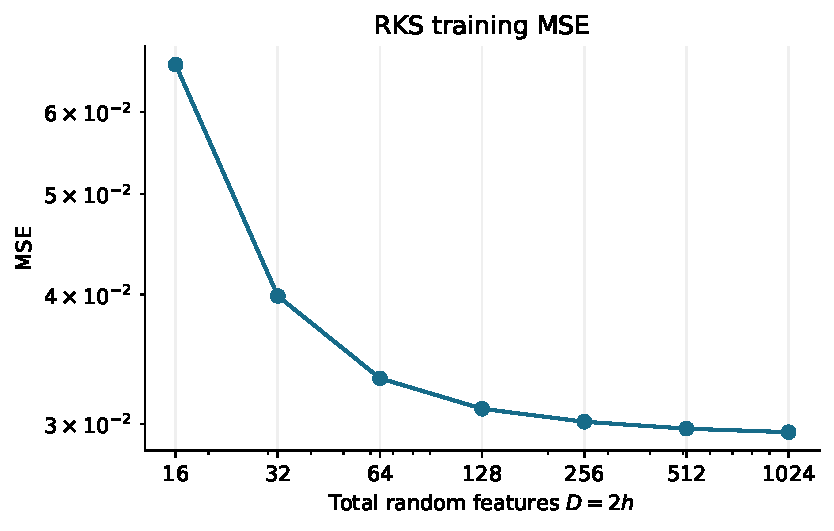
\includegraphics[width=.48\linewidth]{results/figures/q3_rks_train_mse.pdf}\hfill
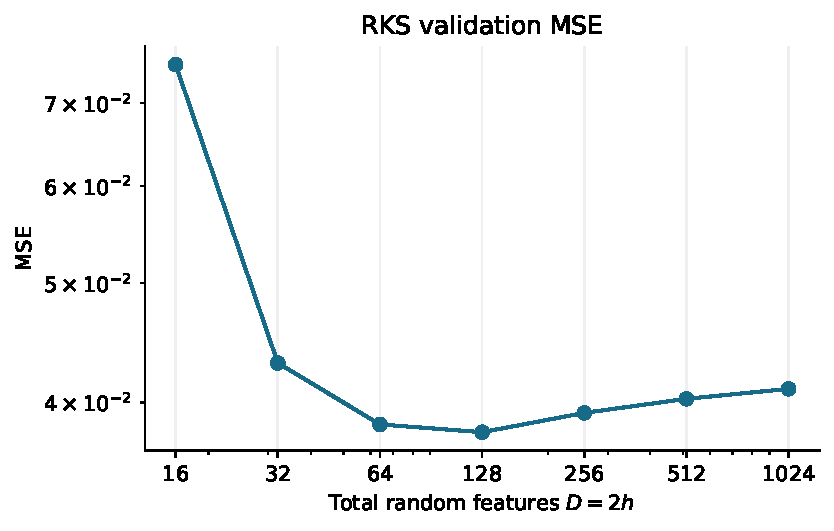
\includegraphics[width=.48\linewidth]{results/figures/q3_rks_validation_mse.pdf}
\end{center}
The two plots show training and validation MSE separately. Increasing the random-feature count lowers training error over the tested range. Validation error falls sharply at first, reaches its minimum at \textbf{$D=\RKSD$ ($h=\RKSPairs$)}, and then rises. The selected count balances approximation and generalization in this sweep. A larger representation can fit training-specific fluctuations even with the ridge coefficient held fixed.

The fixed random features implement a nonlinear basis, while ridge learning is linear in its coefficients and is solved globally. Random frequencies are not adapted to the responses. By contrast, the MLP learns both the basis functions and the output combination. Because these paired features are not normalized by $1/\sqrt h$, $\lambda=0.001$ refers specifically to the stated coefficient penalty and feature convention; numerical values are not directly interchangeable with other RKS normalizations.

\textbf{Selection discipline.} No test responses are available or used. Validation chooses the feature count. The same validation set is used for the MLP sweep, so its eventual comparison is a model-selection result, not an untouched test estimate.

\newpage
\heading{3(c). One-hidden-layer MLP sweep}
The PyTorch model is exactly
\[
 \widehat y=v^\top\tanh(Wx+b)+c,
 \qquad W\in\mathbb R^{H\times2},\quad v,b\in\mathbb R^H.
\]
It has one hidden layer and a linear output. I vary only $H\in\{8,16,32,64,128,256\}$. All other settings are fixed: untransformed inputs/targets, MSE, Adam, learning rate $0.003$, weight decay $10^{-5}$, batch size 128, clipping at gradient norm 10, maximum 3,000 epochs, seed 2026, and validation checks every 10 epochs. Training stops after 250 epochs without improvement and restores the best checked checkpoint. The stopping rule is held fixed; the selected epoch may differ across widths.
\begin{center}\small
\begin{tabular}{lrrr}
\toprule
Hidden width & Selected epoch & Training MSE & Validation MSE \\
\midrule
8 & 2900 & 0.03351232 & 0.03751324 \\
16 & 2340 & 0.03316659 & 0.03572800 \\
32 & 1660 & 0.03210091 & 0.03638932 \\
64 & 920 & 0.03330857 & 0.03718114 \\
128 & 630 & 0.03387519 & 0.03665732 \\
256 & 640 & 0.03308663 & 0.03675643 \\
\bottomrule
\end{tabular}\end{center}

\begin{center}
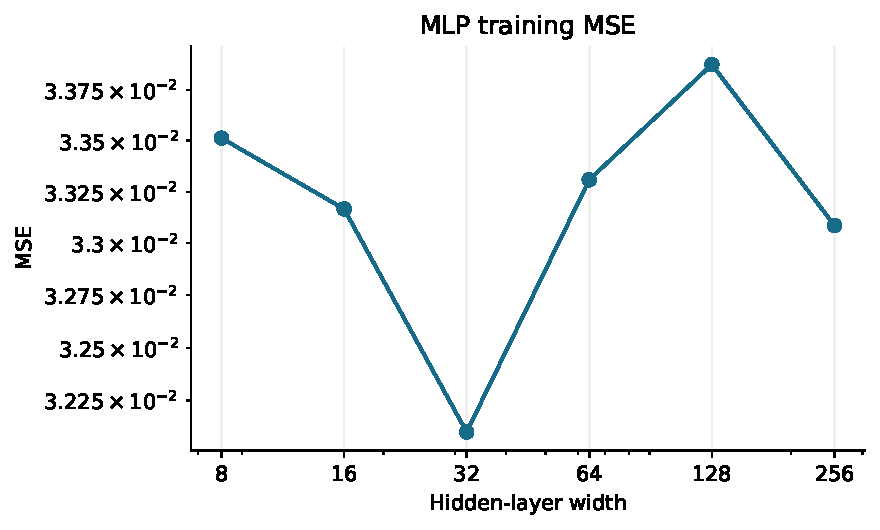
\includegraphics[width=.48\linewidth]{results/figures/q3_mlp_train_mse.pdf}\hfill
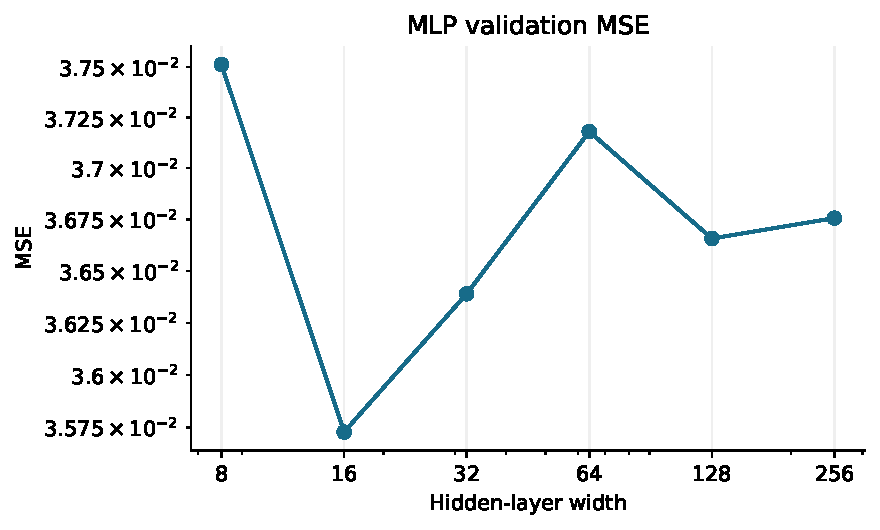
\includegraphics[width=.48\linewidth]{results/figures/q3_mlp_validation_mse.pdf}
\end{center}
The selected model has \textbf{$H=\MLPWidth$}, with checkpoint epoch \MLPEpoch{}. Wider networks do not monotonically improve validation performance. The reported training MSE is evaluated at each width's selected checkpoint, so it need not decline monotonically with width either. The smallest width reaches the 3,000-epoch cap; no claim is made that each nonconvex optimization has found a global minimum.

The hidden functions $\tanh(w_j^\top x+b_j)$ are learned from training labels. This allows the network to adapt a small representation to the observed smooth response structure. It also requires iterative nonconvex optimization and checkpoint selection, unlike the RKS ridge fit. Width, regularization, optimization, and random initialization all affect the result; a single sweep cannot establish a universal advantage for either method.

\newpage
\heading{3(d). Refit, compare, and predict the unlabeled test data}
After selecting hyperparameters, I initialize and fit both models again from scratch on the \emph{training rows only}. The RKS refit uses $D=\RKSD$, $\sigma=1$, and $\lambda=0.001$. The MLP refit uses width \MLPWidth{} for exactly \MLPEpoch{} epochs. With the same seeds, both reproduce their selection validation MSEs. Validation rows remain outside gradient/ridge fitting so the reported validation scores retain their stated meaning.
\begin{center}\small
\begin{tabular}{lrr}
\toprule
Refitted model & Training MSE & Validation MSE \\
\midrule
RKS & 0.03103044 & 0.03783134 \\
MLP & 0.03316659 & 0.03572800 \\
\bottomrule
\end{tabular}\end{center}

The MLP has \MLPImprovement{}\% lower validation MSE than RKS on this fixed split, despite a slightly higher training MSE. Learned features and the selected regularization/stopping combination plausibly match the smooth structure more efficiently here. This is a modest validation advantage, not a measured test advantage or proof of statistical significance.
\begin{center}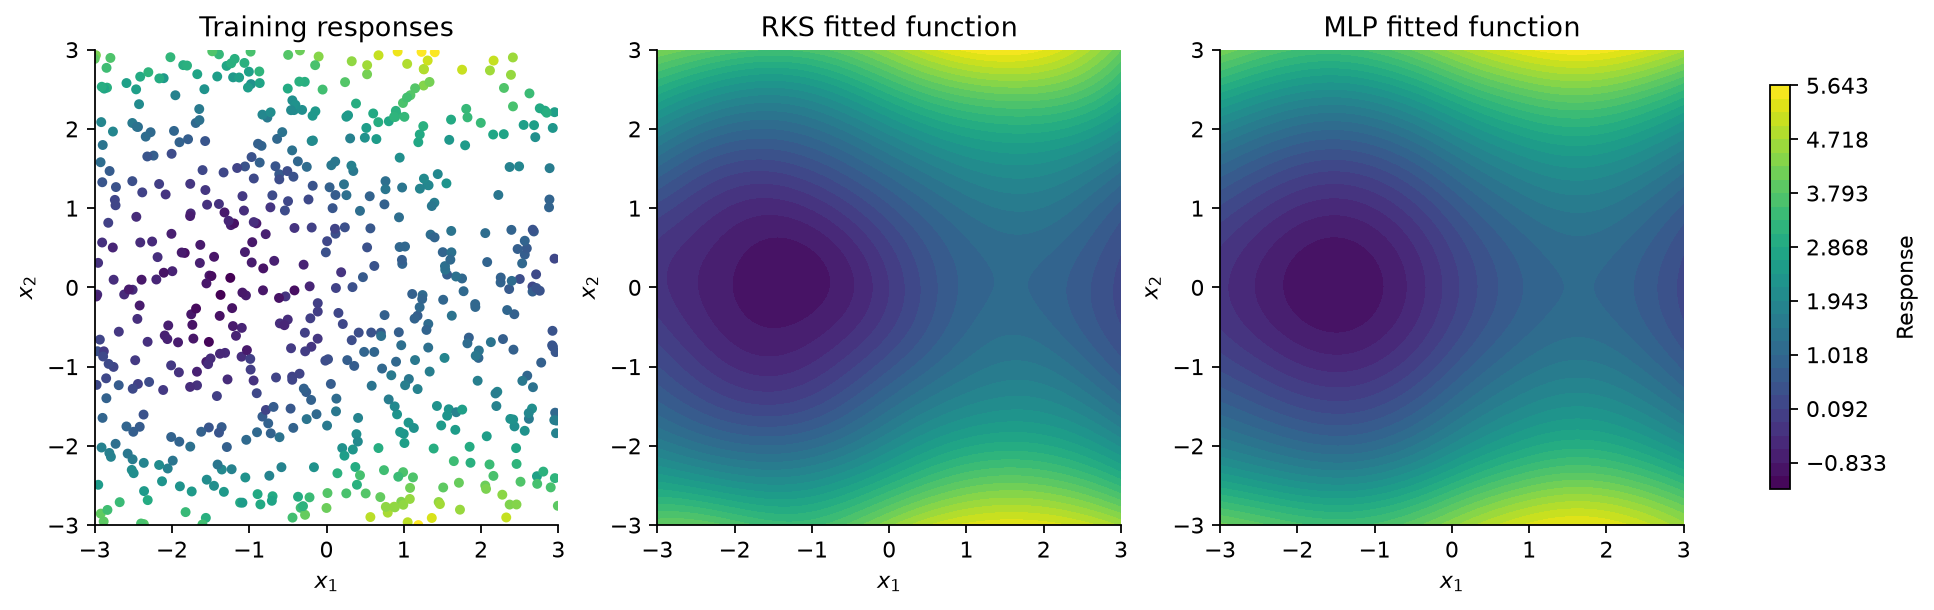
\includegraphics[width=\linewidth]{results/figures/q3_surface_comparison.png}\end{center}
Both fitted functions capture the low region around $(-1.5,0)$, the rise toward $|x_2|\approx3$, and the smooth horizontal modulation visible in the training scatter. The surfaces are very similar at this scale; small local and boundary differences cannot be assigned to bias or noise without the true function. Both smooth over individual observation fluctuations rather than reproducing every point's color. All three panels use a shared color scale over the full $[-3,3]^2$ domain.

\textbf{Test predictions.} Predictions from the refits are written to two files, each with \textbf{200 rows, one numeric value per row, no header}, in exactly the original order of \texttt{test.csv}:
\begin{itemize}
\item \href{https://raw.githubusercontent.com/richard0525/foundations-machine-learning-ai/main/homework_2/results/rks_test_predictions.csv}{\texttt{rks\_test\_predictions.csv}}
\item \href{https://raw.githubusercontent.com/richard0525/foundations-machine-learning-ai/main/homework_2/results/mlp_test_predictions.csv}{\texttt{mlp\_test\_predictions.csv}}
\end{itemize}
The repository's \texttt{q3\_test\_audit.csv} additionally includes row indices and both input coordinates, allowing the prediction order to be checked. \textbf{No test MSE is reported because test labels are absent.}

\end{document}
